% chapter12.tex -- The Complete Algorithm
% Based on the author's UGThesis.docx.

\chapter{The Complete Algorithm}
\label{ch:complete_algorithm}

In this chapter we assemble all the components developed in the preceding chapters into a unified algorithm for generating all triangulations of a biconnected plane graph. 
We first give a high-level overview, then describe the three key innovations, present the complete pseudocode, and finally prove correctness.

\section{Algorithm Overview}
\label{sec:algorithm_overview}

Given a biconnected plane graph \(G\) with \(k\) faces \(F_1, F_2, \dots, F_k\) (ordered arbitrarily), the algorithm performs a depth-first search over a double-layer tree:

\begin{enumerate}
    \item The outer layer recursively processes faces in order. 
    For the current face \(F_i\), we build a local genealogical tree of triangulations that are compatible with the chords already added from previous faces \(F_1, \dots, F_{i-1}\).
    \item The inner layer traverses the local genealogical tree of \(F_i\) using the cycle algorithm (Chapter~\ref{ch:cycle_algorithm}) but with additional pruning based on a global chord set \(S\).
    \item A global chord set \(S\) maintains all chords that have been added along the current exploration path. 
    When we enter a node, we push its chords onto \(S\); when we backtrack, we pop them.
    \item Only triangulations that do not create multi-edges with \(S\) are accepted. 
    Branches that would inevitably lead to multi-edges are pruned using the persistence property of non-root chords.
\end{enumerate}

The algorithm outputs every complete triangulation (when all faces have been processed) exactly once, using \(O(1)\) amortised time per output and \(O(n)\) space.

\section{Three Key Innovations}
\label{sec:innovations}

The algorithm builds upon the Parvez–Rahman–Nakano framework for triconnected graphs but introduces three essential innovations to handle biconnected graphs.

\subsection{Innovation 1: Local Genealogical Trees}
\label{sec:local_trees}

Instead of a single global genealogical tree (which fails for biconnected graphs due to multi-edge conflicts), we construct an independent genealogical tree for each face. 
Each local tree is rooted at a \textbf{safe root triangulation} (see Innovation 2) and is traversed via depth-first search. 
The trees for different faces are nested: after fixing a triangulation of face \(F_i\), we recursively process face \(F_{i+1}\) with the updated global chord set.

\begin{figure}[htbp]
    \centering
    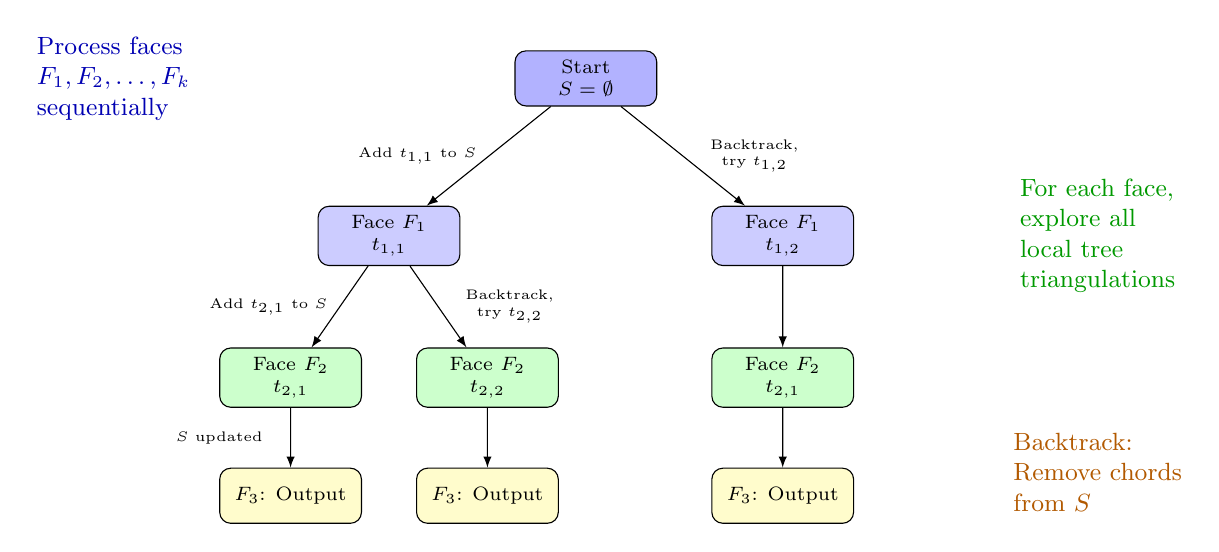
\begin{tikzpicture}[
        level 1/.style={sibling distance=5cm, level distance=2cm},
        level 2/.style={sibling distance=2.5cm, level distance=1.8cm},
        level 3/.style={sibling distance=1.5cm, level distance=1.5cm},
        every node/.style={rectangle, rounded corners, minimum width=1.8cm, minimum height=0.7cm, align=center, font=\scriptsize},
        edge from parent/.style={draw, -latex}
    ]
        \node[draw, fill=blue!30] {Start \\ $S = \emptyset$}
        child {
            node[draw, fill=blue!20] {Face $F_1$ \\ $t_{1,1}$}
            child {
                node[draw, fill=green!20] {Face $F_2$ \\ $t_{2,1}$}
                child {
                    node[draw, fill=yellow!20] {$F_3$: Output}
                    edge from parent node[left, draw=none, font=\tiny] {$S$ updated}
                }
                edge from parent node[left, draw=none, font=\tiny] {Add $t_{2,1}$ to $S$}
            }
            child {
                node[draw, fill=green!20] {Face $F_2$ \\ $t_{2,2}$}
                child {
                    node[draw, fill=yellow!20] {$F_3$: Output}
                }
                edge from parent node[right, draw=none, font=\tiny] {Backtrack,\\ try $t_{2,2}$}
            }
            edge from parent node[left, draw=none, font=\tiny] {Add $t_{1,1}$ to $S$}
        }
        child {
            node[draw, fill=blue!20] {Face $F_1$ \\ $t_{1,2}$}
            child {
                node[draw, fill=green!20] {Face $F_2$ \\ $t_{2,1}$}
                child {
                    node[draw, fill=yellow!20] {$F_3$: Output}
                }
            }
            edge from parent node[right, draw=none, font=\tiny] {Backtrack,\\ try $t_{1,2}$}
        };

        \node[draw=none, font=\small, align=left, blue!70!black] at (-6, 0)
        {Process faces\\$F_1, F_2, \ldots, F_k$\\sequentially};

        \node[draw=none, font=\small, align=left, green!60!black] at (6.5, -2)
        {For each face,\\explore all\\local tree\\triangulations};

        \node[draw=none, font=\small, align=left, orange!70!black] at (6.5, -5)
        {Backtrack:\\Remove chords\\from $S$};
    \end{tikzpicture}
    \caption{Double-layer DFS: outer recursion over faces, inner recursion over triangulations of each face.}
    \label{fig:double_layer_dfs_complete}
\end{figure}

\subsection{Innovation 2: Safe Root Vertex Selection}
\label{sec:safe_root_innovation}

For each face, we must begin with a triangulation that does not conflict with the chords already in \(S\). 
A vertex \(r\) is a \textbf{safe root} if adding all chords \((r, x)\) for non-neighbouring vertices \(x\) on the face introduces no chord that already belongs to \(S\). 
Theorem~\ref{thm:safe_root_exists} guarantees that at least two safe roots exist for any face. 
Chapter~\ref{ch:safe_root_algorithm} gives an \(O(n)\) two-pointer algorithm to find one.

\subsection{Innovation 3: Dynamic Global Chord Management}
\label{sec:global_chord_innovation}

The global chord set \(S\) is implemented as a hash set supporting \(O(1)\) expected insertion, deletion, and membership queries. 
It is updated with push/pop operations during the DFS:

\begin{itemize}
    \item When entering a triangulation node (a specific triangulation of the current face), we insert its chords into \(S\).
    \item When backtracking from that node (after exploring all its descendants), we remove its chords from \(S\).
\end{itemize}

This ensures that \(S\) always contains exactly the chords on the current path from the root of the outer recursion to the current node.

\begin{figure}[htbp]
    \centering
    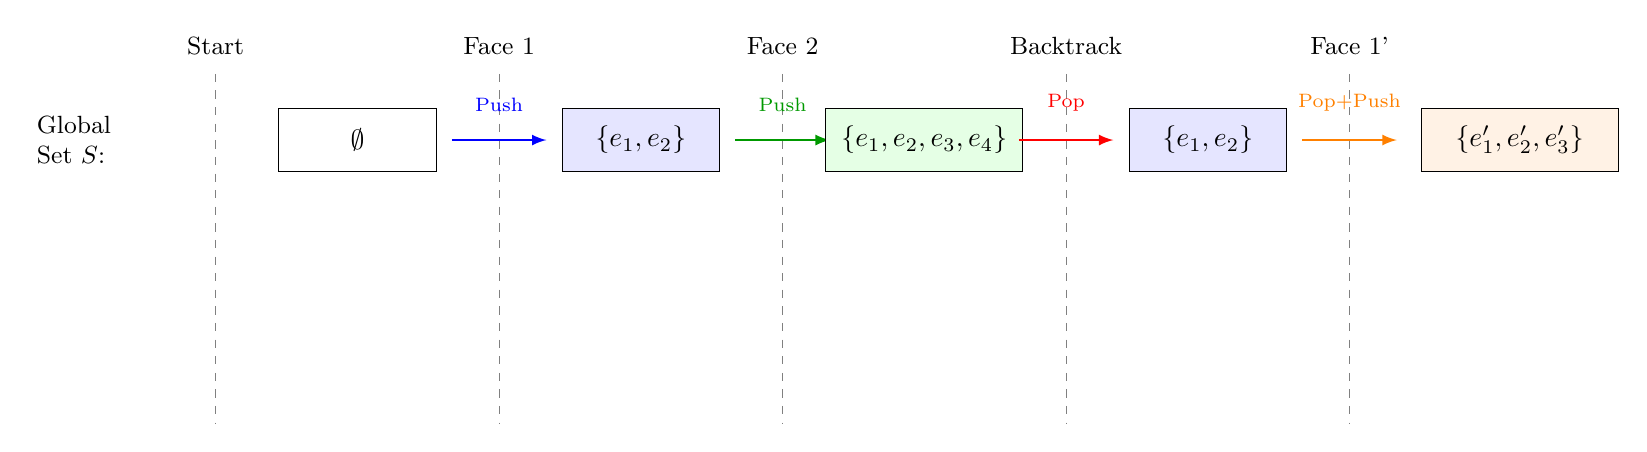
\begin{tikzpicture}[scale=1.2]
        \foreach \x/\label in {0/Start, 3/Face 1, 6/Face 2, 9/Backtrack, 12/Face 1'} {
            \node[font=\small] at (\x, 3.5) {\label};
            \draw[dashed, gray] (\x, 3.2) -- (\x, -0.5);
        }
        \node[draw=none, font=\small, align=left] at (-1.5, 2.5) {Global\\Set $S$:};
        \node[draw, minimum width=2cm, minimum height=0.8cm] at (1.5, 2.5) {$\emptyset$};
        \draw[-latex, thick, blue] (2.5, 2.5) -- (3.5, 2.5);
        \node[draw=none, font=\scriptsize, blue, above] at (3, 2.7) {Push};
        \node[draw, minimum width=2cm, minimum height=0.8cm, fill=blue!10] at (4.5, 2.5) {$\{e_1, e_2\}$};
        \draw[-latex, thick, green!60!black] (5.5, 2.5) -- (6.5, 2.5);
        \node[draw=none, font=\scriptsize, green!60!black, above] at (6, 2.7) {Push};
        \node[draw, minimum width=2.5cm, minimum height=0.8cm, fill=green!10] at (7.5, 2.5) {$\{e_1, e_2, e_3, e_4\}$};
        \draw[-latex, thick, red] (8.5, 2.5) -- (9.5, 2.5);
        \node[draw=none, font=\scriptsize, red, above] at (9, 2.7) {Pop};
        \node[draw, minimum width=2cm, minimum height=0.8cm, fill=blue!10] at (10.5, 2.5) {$\{e_1, e_2\}$};
        \draw[-latex, thick, orange] (11.5, 2.5) -- (12.5, 2.5);
        \node[draw=none, font=\scriptsize, orange, above] at (12, 2.7) {Pop+Push};
        \node[draw, minimum width=2.5cm, minimum height=0.8cm, fill=orange!10] at (13.8, 2.5) {$\{e_1', e_2', e_3'\}$};
    \end{tikzpicture}
    \caption{Dynamic global chord set management with push/pop operations.}
    \label{fig:global_chord_management_complete}
\end{figure}

\section{Building Phase for a Face}
\label{sec:building_phase}

Before traversing the local genealogical tree of a face \(F_i\), we perform the following steps:

\begin{enumerate}
    \item \textbf{Find a safe root vertex} \(v_r\) using the two-pointer algorithm (Chapter~\ref{ch:safe_root_algorithm}). 
    This takes \(O(n_i)\) time, where \(n_i\) is the number of vertices of \(F_i\).
    
    \item \textbf{Build the safe root triangulation} \(T_r\) by adding all chords \((v_r, v_j)\) for every non-neighbouring vertex \(v_j\) on the cycle. 
    This adds \(n_i-3\) chords and initialises the lists \(L\) (all chords), \(GS\) (all root-incident chords), and \(O\) (opposite pairs). 
    This also takes \(O(n_i)\) time.
    
    \item \textbf{Initialise the valid generating set (VGS)}: 
    For each generating chord \((v_r, v_j)\) in \(GS\), compute its opposite pair and check whether it is already in the global set \(S\). 
    If the opposite pair is not in \(S\), add \((v_r, v_j)\) to the VGS. 
    This step is also \(O(n_i)\).
\end{enumerate}

Thus the total building time per face is \(O(n_i)\). 
By the lower bound of \(\Omega(n_i)\) triangulations for that face (Chapter~\ref{ch:lower_bound}), this cost is amortised to \(O(1)\) per output triangulation.

\section{Flipping Phase (Traversing the Local Tree)}
\label{sec:flipping_phase}

After building the root triangulation, we traverse its local genealogical tree in depth-first order. 
The procedure for a triangulation \(T\) of the current face is as follows:

\begin{enumerate}
    \item If the current face is the last face (\(i = k\)), output the complete triangulation (the union of chords from all faces).
    \item Otherwise, recurse to the next face \(F_{i+1}\) with the current set of chords added to \(S\).
    \item Determine the leftmost blocking chord \((v_b, v_{b'})\) of \(T\) (for the root, set \(b' = 3\)).
    \item For each generating chord \((v_r, v_j)\) in the VGS with \(j \ge b'\):
        \begin{itemize}
            \item Flip the chord to obtain a child triangulation \(T'\).
            \item Update the global set \(S\) by inserting the new chord \((v_o, v_{o'})\) (the opposite pair) and removing the flipped chord \((v_r, v_j)\) (which is no longer in the triangulation).
            \item Update the VGS for the affected border chords (at most two chords) by checking their new opposite pairs against \(S\).
            \item Recursively process \(T'\).
            \item Upon returning, backtrack: remove the new chord from \(S\) and re-insert the flipped chord, and restore the VGS of the parent.
        \end{itemize}
\end{enumerate}

All flip and update operations take \(O(1)\) time, as argued in Chapter~\ref{ch:vgs}.

\section{Complete Pseudocode}
\label{sec:pseudocode}

We now present the complete algorithm in a structured pseudocode. 
The global variables are the graph \(G\), the ordered list of faces \(F_1, \dots, F_k\), and the global chord set \(S\) (initially empty).

\begin{algorithm}[htbp]
    \caption{FindAllTriangulations (main)}
    \label{alg:main}
    \begin{algorithmic}[1]
        \Procedure{FindAllTriangulations}{$G$}
            \State $k \gets$ number of faces of $G$
            \State Label faces arbitrarily as $F_1, F_2, \dots, F_k$
            \State $S \gets \emptyset$ \Comment{Global chord set}
            \State \Call{ProcessFace}{$1, \emptyset$}
        \EndProcedure
    \end{algorithmic}
\end{algorithm}

\begin{algorithm}[htbp]
    \caption{ProcessFace (outer recursion)}
    \label{alg:process_face}
    \begin{algorithmic}[1]
        \Procedure{ProcessFace}{$i, T_{\text{prev}}$}
            \If{$i > k$}
                \State \textbf{output} $T_{\text{prev}}$ \Comment{All faces triangulated}
                \State \Return
            \EndIf
            \State $F \gets F_i$
            \State $v_r \gets$ \Call{FindSafeRoot}{$F, S$} \Comment{Two-pointer algorithm}
            \State $T_{\text{root}} \gets$ \Call{BuildRootTriangulation}{$F, v_r$}
            \If{$T_{\text{root}}$ conflicts with $S$} \Comment{Should not happen if $v_r$ is safe}
                \State \Return
            \EndIf
            \State Insert chords of $T_{\text{root}}$ into $S$
            \State $VGS \gets$ \Call{InitVGS}{$T_{\text{root}}, S$}
            \State \Call{DFS}{$T_{\text{root}}, i, VGS, T_{\text{prev}} \cup T_{\text{root}}$}
            \State Remove chords of $T_{\text{root}}$ from $S$ \Comment{Backtrack}
        \EndProcedure
    \end{algorithmic}
\end{algorithm}

\begin{algorithm}[htbp]
    \caption{DFS (inner recursion over local tree)}
    \label{alg:dfs_local}
    \begin{algorithmic}[1]
        \Procedure{DFS}{$T, i, VGS, T_{\text{partial}}$}
            \If{$i = k$}
                \State \textbf{output} $T_{\text{partial}}$ \Comment{Complete triangulation}
            \Else
                \State \Call{ProcessFace}{$i+1, T_{\text{partial}}$}
            \EndIf
            \State Let $(v_b, v_{b'})$ be the leftmost blocking chord of $T$ (if $T$ is root, set $b' = 3$)
            \For{each $(v_r, v_j) \in VGS$ with $j \ge b'$}
                \State $(v_o, v_{o'}) \gets$ opposite pair of $(v_r, v_j)$
                \State $T' \gets$ \Call{Flip}{$T, (v_r, v_j)$} \Comment{Remove $(v_r, v_j)$, add $(v_o, v_{o'})$}
                \State Insert $(v_o, v_{o'})$ into $S$, remove $(v_r, v_j)$ from $S$
                \State Update $VGS'$ from $VGS$ for the affected border chords
                \State \Call{DFS}{$T', i, VGS', T_{\text{partial}} \cup \{(v_o, v_{o'})\}$}
                \State Restore $S$ and $VGS$ (backtrack)
            \EndFor
        \EndProcedure
    \end{algorithmic}
\end{algorithm}

The subroutines \textsc{FindSafeRoot} (Chapter~\ref{ch:safe_root_algorithm}), \textsc{BuildRootTriangulation} (Chapter~\ref{ch:cycle_algorithm}), and \textsc{InitVGS} (Chapter~\ref{ch:vgs}) have been described previously.

\section{Correctness Proof}
\label{sec:correctness_complete}

We now prove that the algorithm generates every valid triangulation exactly once and outputs only valid triangulations.

\begin{theorem}[Completeness]
    \label{thm:completeness_final}
    The algorithm generates all triangulations of the input biconnected plane graph \(G\) without duplication.
\end{theorem}

\begin{proof}
    The proof proceeds by induction on the number of faces.

    \textbf{Base case:} A graph with one face (a cycle). 
    The algorithm reduces to the cycle algorithm of Chapter~\ref{ch:cycle_algorithm}, which is known to generate all triangulations without duplication (Parvez et al.~\cite{parvez2011}).

    \textbf{Inductive step:} Assume the algorithm correctly generates all triangulations for graphs with at most \(k-1\) faces. 
    Consider a graph with \(k\) faces \(F_1, \dots, F_k\). 
    For a fixed triangulation \(T_1\) of \(F_1\) that is compatible with \(S = \emptyset\) (i.e., contains no chords from previous faces — trivially true), we recursively generate all triangulations of the subgraph formed by faces \(F_2, \dots, F_k\) with the chords of \(T_1\) added to \(S\). 
    By the induction hypothesis, this yields all completions of \(T_1\) to a full triangulation of \(G\). 
    The outer loop over all triangulations of \(F_1\) (generated by the local DFS) therefore produces every combination. 
    Duplications cannot occur because the local genealogical tree for \(F_1\) is free of duplicates, and the recursion for the remaining faces is applied independently for each \(T_1\).

    The pruning condition (skipping a child when its opposite pair is already in \(S\)) eliminates only those branches that would inevitably contain a multi-edge (Lemma~\ref{lem:pruning_opposite}). 
    Hence no valid triangulation is lost.
\end{proof}

\begin{theorem}[No invalid triangulations]
    \label{thm:no_invalid}
    Every triangulation output by the algorithm is a valid triangulation of \(G\) (i.e., contains no multi-edges).
\end{theorem}

\begin{proof}
    The algorithm only adds a chord \((v_o, v_{o'})\) to a triangulation when flipping a generating chord \((v_r, v_j)\) whose opposite pair is not in \(S\). 
    By the invariant that \(S\) contains all chords from previous faces and from the current partial triangulation along the path, the new chord does not already exist. 
    Moreover, when a chord is added, it never creates a crossing because all chords are added inside a single face and planarity is preserved by the flip operation. 
    Thus every intermediate and final triangulation is simple and planar.
\end{proof}

\section{Summary}
\label{sec:complete_summary}

We have assembled all components into a complete algorithm for generating all triangulations of a biconnected plane graph. 
The algorithm processes faces sequentially, uses a global chord set to avoid multi-edges, finds a safe root in linear time, and maintains a valid generating set to enable constant-time flips. 
Correctness follows from the properties of the genealogical tree and the pruning lemma. 
The next chapter analyses the time and space complexity, proving \(O(1)\) amortised time per triangulation and \(O(n)\) space.